\chapter{'വരവില' എന്ന നുകം രൂപമെടുക്കുന്നു}
\label{chapter5}

\begin{figure}[h]
\begin{center}
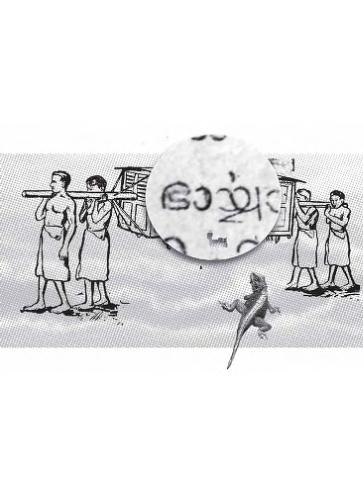
\includegraphics[width=0.5\textwidth,height=8cm]{Kulasthree_Chapter_five_pic01.jpg}
\end{center}
%\caption*{പുലയർ - കെ പി പത്മനാഭ മേനോൻ - വാള്യം 3, (1929), 1984}
\end{figure}

സ്ത്രീധനത്തെക്കുറിച്ച് വേവലാതിപ്പെടാത്ത കുടുംബങ്ങൾ ഇന്ന് കേരളത്തിൽ കുറവാണ്. എന്നാൽ ഈ സമ്പ്രദായം നാട്ടിലാകെ പടർന്നുപിടിച്ചത് അൽപകാലം മുമ്പുമാത്രമാണെന്നതാണ് വാസ്തവം. മാത്രമല്ല, ഇന്ന് 'സ്ത്രീക്കു നൽകുന്ന ധന'മല്ല സ്ത്രീധനം - 'വരനു നൽകുന്ന വില'യാണ്. വിവാഹസ്ഥിരതയെക്കുറിച്ചും കുടുംബത്തിൽ ഭർത്താവിന്റെ അധികാരങ്ങളെക്കുറിച്ചുമുള്ള ധാരണകളിലുമുണ്ടായ മാറ്റങ്ങളിൽനിന്നാണ് സ്ത്രീധനമേർപ്പാട് രൂപപ്പെട്ടത്. സാമൂഹ്യമാറ്റത്തിനിടയിൽ ഉയർന്നുവന്ന തിന്മയാണ് സ്ത്രീധനമെന്നു തിരിച്ചറിയുമ്പോൾ സാമൂഹ്യമാറ്റത്തിലൂടെ അതിനെ ഇല്ലായ്മചെയ്യാനാകുമെന്നതിനെക്കുറിച്ചുള്ള ആത്മവിശ്വാസവും വർദ്ധിക്കുന്നു.

\section{'സ്ത്രീധനം' അല്ല!}
\label{ch5sec1}

\paragraph{}തുടക്കത്തിൽത്തന്നെ പറയാം, കേരളത്തിൽ വിവാഹങ്ങളോടനുബന്ധിച്ച് നടക്കുന്ന കൊടുക്കൽവാങ്ങലിന് 'സ്ത്രീധനം' എന്ന പേർ യോജിക്കില്ല. കല്യാണവേളയിൽ വധുവിന് സ്വന്തം കുടുംബം നൽകുന്ന സമ്മാനമാണ് 'സ്ത്രീധനം'. അതവൾക്ക് നേരിട്ടവകാശപ്പെട്ടതും സ്വന്തമായി കൈകാര്യം ചെയ്യാവുന്നതുമായ മുതലാണ്. എന്തെങ്കിലും കാരണവശാൽ അവൾക്ക് വിവാഹബന്ധം ഒഴിയേണ്ടിവന്നാൽ സ്ത്രീധനം മടക്കിക്കൊടുക്കാൻ ഭർത്താവിന്റെ വീട്ടുകാർ ബാദ്ധ്യസ്ഥരുമാണ്. പക്ഷേ കേരളത്തിൽ ഇന്നു നിലവിലുള്ള രീതി ഇതല്ല; അത് 'വരവില'യാണ് - വധുവിന്റെ വീട്ടുകാർ വരന്റെ 'യോഗ്യത'യനുസരിച്ച് അയാൾക്കു നൽകുന്ന ധനം - വരന്റെ 'യോഗ്യത'യനുസരിച്ച് അത് കൂടിയും കുറഞ്ഞുമിരിക്കും. വധുവിന്റെ 'യോഗ്യത'യും പരിഗണിക്കാറുണ്ടെങ്കിലും അതിനു താരതമ്യേന പ്രാധാന്യം കുറവാണ്.

\paragraph{}ഇന്ന് കേരളത്തിലെ താണ-ഇടത്തരം കുടുംബങ്ങളെ ദാരിദ്യ്രത്തിലേക്കു വലിച്ചിഴക്കുന്ന പ്രധാന കാരണങ്ങൾ രണ്ടാണ്. ഒന്ന് ചെലവേറിയ ചികിത്സ ആവശ്യമായിവരുന്ന രോഗങ്ങൾ; രണ്ട്, പെൺകുട്ടികളെ എന്തു നഷ്ടവും സഹിച്ച് 'അയയ്ക്കണം' എന്ന ചിന്ത. ആദ്യത്തേതിനുമേൽ നമുക്കധികം നിയന്ത്രണം ഒരുപക്ഷേ ഇല്ലായിരിക്കാം. രണ്ടാമത്തേത് നാംതന്നെ വരുത്തിവയ്ക്കുന്നതാണ്. ആൺകുട്ടികളെപ്പോലെയോ അവരെക്കാൾ മെച്ചമായോ പഠിക്കാനും ജോലിചെയ്യാനും സമ്പാദിക്കാനും പെൺകുട്ടികൾക്കു കഴിയുമെന്ന് ഇന്നു നമുക്കറിയാം. പഠിത്തം, ജോലി, ഇവയിലേക്കു കടക്കാൻ പെൺകുട്ടികളെ നാം പ്രാത്സാഹിപ്പിക്കുന്നുമുണ്ട്. എന്നാൽ ഇതിലൊക്കെ അധികമാണ് പെൺകുട്ടികളെ വിവാഹം കഴിപ്പിക്കാനുള്ള പരിശ്രമം! പഠിച്ചുവളർന്ന പെൺകുട്ടി ആത്മാഭിമാനമുള്ള, മുതിർന്ന, ഒരു വ്യക്തിയാണെന്ന കാര്യത്തെപ്പോലും അവഗണിച്ചുകൊണ്ട് ഏതുവിധേനയും ഒരു വരനെക്കണ്ടെത്താൻ മാതാപിതാക്കന്മാർ ശ്രമിക്കും. ഒടുവിൽ വലിയ വിലകൊടുത്ത് ഒരാളെ കൊണ്ടുവരും. അതും ഒരു ഭാഗ്യപരീക്ഷണംമാത്രമാണ്. നന്നായില്ലെങ്കിൽ 'അവളുടെ തലയിലെഴുത്ത്' എന്ന് ദീർഘമായി നിശ്വസിക്കും; ആ അദ്ധ്യായം അടയ്ക്കും. പിന്നെ ആ സാധുപെൺകുട്ടിയുടെ നശിച്ചുപോയ ജീവിതം അവളുടെമാത്രം തലവേദനയാണ്.


\captionof{mybox}{കേരളത്തിലെ മിഷണറിസഭകൾ}
\label{ch5box1} % place the caption
\begin{tcolorbox}[%
 breakable, % make the box breakable
  arc=0mm, 
  left=1pt, right = 1pt, 
  boxrule=0mm,
  colback = {blue!10}, % since shadow-gray was not defined
] 


ചർച്ച് മിഷണറി സൊസൈറ്റി (CMS), ലണ്ടൻ മിഷണറി സൊസൈറ്റി (LMS), ബാസൽ മിഷൻ (Basel Mission) എന്നീ മൂന്നു സഭകളാണ് 19-ാം നൂറ്റാണ്ടുമുതൽ കേരളത്തിൽ പ്രേഷിതവേലയിൽ ഏർപ്പെട്ടത്. ഇവയിൽ ആദ്യത്തെ രണ്ട് സഭകൾ കേരളത്തിന്റെ തെക്കൻഭാഗങ്ങളിലും ബാസൽമിഷൻ വടക്കൻ കേരളത്തിലും പ്രവർത്തിച്ചു. 19-ാം നൂറ്റാണ്ടിൽ തിരുവിതാംകൂറിൽ ബ്രിട്ടിഷ് അധികാരത്തിന് അടിസ്ഥാനമിട്ട കേണൽ മൺറോയുടെ ഒത്താശയോടെയാണ് മിഷണറിപ്രവർത്തകർ ഈ നാട്ടിൽ ചുവടുറപ്പിച്ചത്. എന്നാൽ മതംമാറ്റുക എന്ന ഒരൊറ്റ ജോലിമാത്രമല്ല മിഷണറിമാർ ചെയ്തത്. ജാതിവ്യത്യാസങ്ങൾക്കപ്പുറത്ത് എല്ലാവർക്കും വിദ്യാഭ്യാസം നൽകിയിരുന്ന വിദ്യാലയങ്ങൾ ഈ നാട്ടിലാരംഭിച്ചത് അവരാണ്. കീഴാളർക്ക് വിദ്യയുടെ വെളിച്ചം എത്തിച്ചുകൊടുക്കുകവഴി നിലവിലുണ്ടായിരുന്ന ജാത്യാചാരത്തിലെ അനീതിയെയും അക്രമത്തെയും പ്രത്യക്ഷത്തിലെതിർക്കാനുള്ള ധൈര്യവും അവർ പകർന്നു. 1850കൾവരെ തെക്കൻ തിരുവിതാംകൂറിലെ നാടാന്മാർ ഉന്നതജാതിക്കാർക്കെതിരെ നടത്തിയ മാറുമറയ്ക്കൽ സമരത്തിന് ഉറച്ച പിന്തുണ നൽകിയത് LMS പാതിരിമാരായിരുന്നു. എല്ലാ ജാതിമതക്കാരും ഒന്നിച്ചു പഠിച്ച, ഉന്നതനിലവാരം പുലർത്തിയ, നിരവധി സ്കൂളുകളും കലാലയങ്ങളും അവർ സ്ഥാപിക്കുകയുണ്ടായി. വടക്ക് ബാസൽമിഷനാകട്ടെ, പല പുതിയ തൊഴിലുകളും ജനങ്ങളെ പരിശീലിപ്പിച്ചു. മലയാളഭാഷയ്ക്കും കനത്ത സംഭാവനകൾ മിഷണറിമാരിൽനിന്നുണ്ടായിട്ടുണ്ട്. ഹെർമ്മൻ ഗുണ്ടർട്ട്, ബെഞ്ചമിൻ ബെയ്ലി എന്നീ നാമങ്ങൾ മലയാളഭാഷാചരിത്രത്തിൽ തിളങ്ങിനിൽക്കുന്നവയാണ്.

\end{tcolorbox}

\paragraph{}എന്നാൽ പഴയകാലത്ത് സ്ത്രീധനം കൊടുക്കുന്നവർക്ക് വിവാഹബന്ധം ഒഴിഞ്ഞാൽ അതു മുഴുവനായോ ഭാഗികമായോ മടക്കിക്കിട്ടാനുള്ള സംവിധാനം പല സമുദായങ്ങളിലുമുണ്ടായിരുന്നു. വിവാഹസമയത്ത് കിട്ടുന്ന സമ്മാനങ്ങളുടെ കണക്ക് കൃത്യമായി എടുത്തുവയ്ക്കുന്ന രീതി ഇന്നും പല സമുദായങ്ങളിലുമുണ്ട്. ഈ പഴുതുകളെല്ലാം ഇരുപതാംനൂറ്റാണ്ടിൽ ചുരുങ്ങുകയാണുണ്ടായത്. വരവിലയുടെ സ്വാധീനം വളരുംതോറും ഇന്ന് നിലവിലുള്ളവയുടെ ആയുസ്സു കുറയുമെന്നു തീർച്ചയാണ്. 20-ാംനൂറ്റാണ്ടിന്റെ പ്രത്യേകത അതുമാത്രമല്ല. മുമ്പ് സ്ത്രീധനസമ്പ്രദായം തീരെ പതിവില്ലായിരുന്ന സമുദായങ്ങളിലേക്ക് വരവില കടന്നുകയറിയതാണ് 20-ാം നൂറ്റാണ്ടിന്റെ സവിശേഷത.



\paragraph{}'വരവില'യുടെ വരവിനെക്കുറിച്ചാണ് ഈ അദ്ധ്യായം. ഇത്തിൾക്കണ്ണിപോലെ എല്ലാ സമുദായങ്ങളിലും - പണക്കാർ, പാവപ്പെട്ടവർ എന്ന വ്യത്യാസമൊന്നും കൂടാതെ - കയറിപ്പറ്റിയ ഈ ഏർപ്പാട് കേരളത്തിലെ മൊത്തം സ്ത്രീകളും നേരിടുന്ന വിപത്തായിത്തീർന്നിരിക്കുന്നുവെന്നത് പരിഗണിച്ചാണ് അതിനിവിടെ ഇത്രയും പ്രാധാന്യം കല്പിച്ചിരിക്കുന്നത്. ചില ചെറിയ ആദിവാസിഗോത്രങ്ങളിലൊഴിച്ച് മറ്റെല്ലായിടത്തും 'വരവില' പടർന്നുപിടിച്ചിരിക്കുന്നു. മുമ്പാണെങ്കിൽ മലയാളബ്രാഹ്മണർ, ക്രിസ്ത്യാനികൾ തുടങ്ങിയ മക്കത്തായ സമുദായങ്ങൾക്കിടയിലായിരുന്നു സ്ത്രീധനമേർപ്പാട് പൂർണ്ണരീതിയിൽ നിലനിന്നിരുന്നത്. എന്നാൽ 19-ാം നൂറ്റാണ്ടിൽപ്പോലും 'സ്ത്രീധനം' 'വരവില' തന്നെയായിരുന്നില്ലേ എന്നു സംശയിക്കാൻ വകയുണ്ട്. 1822ൽ തിരുവിതാംകൂറിലെ റാണി ഗൗരിപാർവ്വതീഭായി ഒപ്പുവച്ച ഒരു ഉത്തരവുപ്രകാരം ഇവിടത്തെ നമ്പൂതിരി-പോറ്റി സമുദായങ്ങളുടെ സ്ത്രീധനമേർപ്പാടിനുമേൽ നിയന്ത്രണമേർപ്പെടുത്താൻ സർക്കാർ ശ്രമിച്ചതായി കാണുന്നു. ക്രമാതീതമായി വർദ്ധിച്ച സ്ത്രീധനത്തുകമൂലം ബ്രാഹ്മണസ്വത്തുക്കൾ നശിക്കുന്നെന്നും അവിവാഹിതകളായിനിൽക്കുന്ന സ്ത്രീകൾക്ക് പലവിധ ദോഷങ്ങളും ഉണ്ടാകുന്നുവെന്നും ഉത്തരവിൽ പറയുന്നു. സ്ത്രീധനത്തുക നിശ്ചയിച്ചതിനുപുറമെ 14 വയസ്സിലധികം പ്രായമായ കന്യകമാരുടെ വിവാഹം ഉടൻതന്നെ നടത്തിക്കൊള്ളണമെന്നും ഉത്തരവിൽ പറഞ്ഞിരിക്കുന്നു! വരന്മാരുടെ വിലയായിരുന്നു ഇവിടെ സ്ത്രീധനം എന്നു കരുതാൻ കാരണമുണ്ട്; ബ്രഹ്മസ്വങ്ങൾ നശിക്കാൻമാത്രം ഉയർച്ചയാണ്. തുകയിലുണ്ടായത്! ഇതുപോലെ കോട്ടയത്തെ സുറിയാനിക്രിസ്ത്യാനികളുടെ ഗൃഹജീവിതവുമായി തനിക്കുണ്ടായിരുന്ന പരിചയത്തെ അടിസ്ഥാനമാക്കി സി.എം.എസ്. മിഷണറിസഭയിൽ പ്രവർത്തിച്ചിരുന്ന മിഷണറിയായിരുന്ന കോളിൻസ് മദാമ്മ 1877ൽ പ്രസിദ്ധീകരിച്ച ഘാതകവധം എന്ന നോവലിലും 'സ്ത്രീധനം' 'വരവില'യായിരുന്നുവെന്ന് സൂചനയുണ്ട്. പുരുഷന്റെ യോഗ്യതകൾക്ക് കൊടുത്ത അമിത പ്രാധാന്യവും സ്ത്രീയുടെ യോഗ്യതകളെ ഇടിച്ചുതാഴ്ത്താനുമുള്ള പ്രവണതയും ഈ നോവലിൽ വിമർശിക്കപ്പെടുന്നു. 'നല്ല കുടുംബ'മെന്ന യോഗ്യതയുള്ള വരനെ തന്റെ മകൾക്കു കിട്ടണമെങ്കിൽ ഒത്തിരി നിലം പുരയിടങ്ങൾ സമ്പാദിച്ചുകൂട്ടിയേ പറ്റൂ എന്നു വിശ്വസിച്ച കോശീകുര്യൻ എന്നയാളുടെ മനസ്സിനെ മകളായ മറിയം മാറ്റിയെടുത്തതിന്റെ കഥയാണ് ഘാതകവധം പറയുന്നത്.


\begin{figure}[h]
\begin{center}
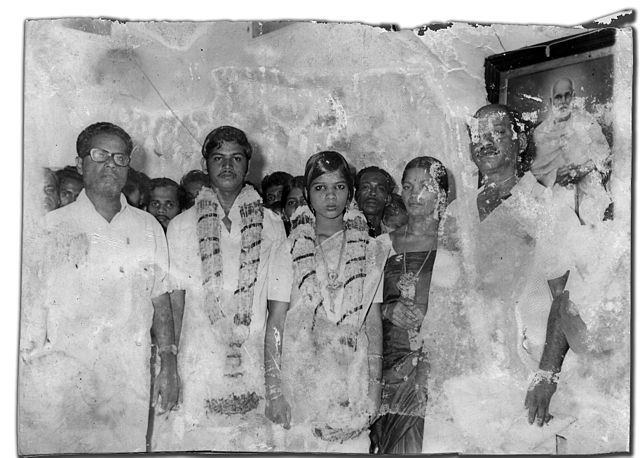
\includegraphics[width=\textwidth,height=8cm]{Kulasthree_Chapter_five_pic02.jpg}
\end{center}
%\caption*{പുലയർ - കെ പി പത്മനാഭ മേനോൻ - വാള്യം 3, (1929), 1984}
\end{figure}

\section{വരവില മാന്യമാകുന്നു}
\label{ch5sec2}
\paragraph{}
അമ്മവഴിക്ക് സ്വത്തവകാശം കണക്കാക്കിയിരുന്ന മരുമക്കത്തായ സമുദായങ്ങളിൽ വരവിലയ്ക്ക് അനുകൂലമായ വിവാഹസമ്പ്രദായമല്ല നിലനിന്നിരുന്നത്. സ്ത്രീക്ക് സ്വന്തം കുടുംബവുമായുള്ള ബന്ധം ഈ സമുദായങ്ങളിൽ വളരെ ശക്തമായിരുന്നു. ഭർത്താവിന്റെ വീട്ടിലാണ് താമസമെങ്കിലും ജനിച്ചവീട്ടിൽനിന്ന് സ്ത്രീ ഒരിക്കലും അകന്നുപോയിരുന്നില്ല. പിറന്നകുടുംബത്തിൽ സ്ത്രീക്കുള്ള ധനപരവും ധാർമ്മികവുമായ അവകാശങ്ങൾ വിവാഹത്തിനുശേഷവും നിലനിന്നുവെന്ന് സാരം. രണ്ടാമതായി, 'മുറച്ചെറുക്ക'നെയോ 'മുറപ്പെണ്ണി'നെയോ (അമ്മാവന്റെ മകൻ, മകൾ അങ്ങനെയുള്ളവരെ) വിവാഹംചെയ്യുന്ന രീതി ഇക്കൂട്ടർക്കിടയിൽ നിലവിലുണ്ടായിരുന്നതുകൊണ്ട് പലപ്പോഴും കല്യാണംകഴിക്കുന്ന പുരുഷൻ അന്യനായിരുന്നില്ല. തന്നെയുമല്ല, വിവാഹമോചനവും വിധവാവിവാഹവും സാധാരണകാര്യങ്ങളായി അംഗീകരിക്കപ്പെട്ടിരുന്നു. ഭാര്യയുടെ സംരക്ഷണത്തിന്റെ ചുമതല അധികവും അവളുടെ സ്വന്തം വീടിനുതന്നെയായിരുന്നതുകൊണ്ട് വിവാഹമോചനംമൂലം സ്ത്രീ തകർന്നുപോകുന്ന ഇന്നത്തെയവസ്ഥ ഉണ്ടായിരുന്നില്ല. കീഴ്ജാതിക്കാർക്കിടയിലാകട്ടെ, വിവാഹസമയത്ത് ചെറുക്കൻവീട്ടുകാർ പെൺവീട്ടുകാർക്ക് 'പെൺപണം' കാഴ്ചവയ്ക്കുന്നരീതി 19-ാം നൂറ്റാണ്ടിലുണ്ടായിരുന്നു. പരമ്പരാഗത മരുമക്കത്തായ കുടുംബങ്ങളിലെ സ്ത്രീകൾ എല്ലാവിധത്തിലും സ്വതന്ത്രകളായിരുന്നു എന്നല്ല പറഞ്ഞുവരുന്നത്. അമ്മാവന്മാരുടെയും ആങ്ങളമാരുടെയും വാക്കിനു കീഴ്വഴങ്ങിയാണ് സ്ത്രീകൾ കഴിഞ്ഞത്; പ്രായമേറിയ സ്ത്രീകൾക്ക്, വിശേഷിച്ച് അമ്മമാർക്ക്, പക്ഷേ, വളരെ മാന്യമായ സ്ഥാനവും കുടുംബത്തിന്റെ സ്വത്തുക്കൾ, പണമിടപാടുകൾ, വരുമാനം എന്നിവയെക്കുറിച്ചുള്ള തീരുമാനങ്ങളിൽ വലിയ പങ്കുമുണ്ടായിരുന്നു. മറ്റൊരുവിധത്തിൽപ്പറഞ്ഞാൽ, ഇന്നത്തെപ്പോലെ 'സ്നേഹത്തിന്റെ അധികാരം' മാത്രമായിരുന്നില്ല അമ്മമാരുടേത്. മലബാറിൽ 19-ാം നൂറ്റാണ്ടിന്റെ അവസാനകാലത്തും 20-ാം നൂറ്റാണ്ടിന്റെ തുടക്കത്തിലും ഗവേഷണം നടത്തിയ എഫ്. ഫാസറ്റ് (F. Fawcett) എന്ന നരവംശശാസ്ത്രജ്ഞൻ തന്റെ Nayars of Malabar (1901) എന്ന പുസ്തകത്തിൽ ഇവിടെ നിലവിലുണ്ടായിരുന്ന 'സംബന്ധവ്യവസ്ഥ'യെക്കുറിച്ച് ഇങ്ങനെയാണ് നിരീക്ഷിച്ചത്:


\begin{quotation}
എല്ലാ ലൈംഗികകാര്യങ്ങളിലും സ്ത്രീകൾക്കും പുരുഷന്മാർക്കും തുല്യസ്വാതന്ത്ര്യം അനുവദിക്കുന്നുവെന്നത് മരുമക്കത്തായവ്യവസ്ഥയുടെ അപൂർവ്വഗുണങ്ങളിലൊന്നുതന്നെ. ഒറ്റരാത്രിമാത്രമേ ഒന്നിച്ചു കഴിഞ്ഞുള്ളു എന്നാലും ഇരുകൂട്ടർക്കും പിരിഞ്ഞുപോകാൻ അനുവാദമുണ്ട്. ലൈംഗികതാത്പര്യം ഇല്ലാതിരിക്കുകയോ മറ്റുവിധത്തിലുള്ള മനഃപൊരുത്തം നഷ്ടമാവുകയോ ചെയ്താൽ ഇരുകൂട്ടർക്കും ബന്ധം വേർപെടുത്തി മറ്റുബന്ധങ്ങളിൽ ഏർപ്പെടാനുള്ള സ്വാതന്ത്ര്യമുണ്ടായിരുന്നു. ഇത് നിത്യവും ബന്ധം പിരിയാനുള്ള പ്രവണതയിൽ കലാശിക്കില്ലേ എന്ന സംശയമുണ്ടാകിനിടയുള്ളതുകൊണ്ട്, അത്തരത്തിലുള്ള യാതൊന്നും ഉണ്ടാവില്ലെന്നകാര്യം ഇവിടെ എടുത്തുപറയട്ടെ. വെറുതെയുള്ള വിവാഹമോചനം അപൂർവ്വമാണ്. സ്ഥിരവിവാഹമാണ് പതിവുരീതി. തറവാട്ടുസ്വത്ത് സ്ത്രീകളെയും അവരുടെ സന്തതികളെയും സംരക്ഷിക്കാനായി നീക്കിവയ്ക്കുന്ന രീതിയാണ് ഈ സമ്പ്രദായത്തിന്റെ അടിത്തറ എന്നു തോന്നുന്നു.
\flushright{(Nayars of Malabar, New Delhi. 1985, പുറം 236-37)}
\end{quotation}

\captionof{mybox}{ 'താലികെട്ടി അമ്മയായി'}
\label{ch5box2} % place the caption
\begin{tcolorbox}[%
 breakable, % make the box breakable
  arc=0mm, 
  left=1pt, right = 1pt, 
  boxrule=0mm,
  colback = {blue!10}, % since shadow-gray was not defined
] 

മരുമക്കത്തായികൾക്കിടയിൽ വിവാഹച്ചടങ്ങിനെക്കാളധികം പ്രാധാന്യം 'താലികെട്ടുകല്യാണം' എന്ന ചടങ്ങിനായിരുന്നു. മാസമുറയെത്തുംമുമ്പ് പെൺകുട്ടികളെ ഏതെങ്കിലും ബ്രാഹ്മണനെക്കൊണ്ടോ സമുദായത്തിലെതന്നെ പ്രമുഖരായവരെക്കൊണ്ടോ താലികെട്ടിക്കുന്ന ചടങ്ങായിരുന്നു നായന്മാർക്കിടയിലുണ്ടായിരുന്നത്. ഇതുകൊണ്ട് പെൺകുട്ടി അയാളുടെ ഭാര്യയായി എന്നർത്ഥമാകുന്നില്ല - ബാല്യത്തിൽനിന്ന് യൗവ്വനത്തിലേക്ക് അവൾ കടന്നുവെന്ന് പ്രഖ്യാപിക്കുന്ന ചടങ്ങുമാത്രമായിരുന്നു ഇത്. എന്നാൽ വളരെ നീണ്ടതും ചിലവേറിയതുമായ ആഘോഷമായിരുന്നതുകൊണ്ട് തറവാട്ടിൽ ആ പ്രായത്തിനടുത്തെത്തിയ പെൺകുട്ടികളുടെ താലികെട്ടുകല്യാണം ഒരുമിച്ചുനടത്തുന്ന രീതി പതിവായിരുന്നു. താലികെട്ടിക്കഴിഞ്ഞ പെൺകുട്ടി 'അമ്മയായി' എന്നായിരുന്നു ചൊല്ല്. മക്കത്തായികളായ ഈഴവർക്കിടയിൽ താലികെട്ട് നിർവ്വഹിച്ചിരുന്നത് അന്യപുരുഷന്മാരായിരുന്നില്ല; ഏതെങ്കിലും സ്ത്രീയായിരുന്നു അത് നിർവ്വഹിച്ചിരുന്നത്. സാമ്പത്തികസ്ഥിതി ഇല്ലാത്ത കുടുംബങ്ങൾ അതു ചെറിയതോതിൽ നടത്തിയിരുന്നു- പെൺകുട്ടിയുടെ അമ്മതന്നെ താലികെട്ടുകയോ ഒരു ബൊമ്മയെ അടുത്തിരുത്തിയശേഷം ഏതെങ്കിലും സ്ത്രീകളായ ബന്ധുക്കൾ താലികെട്ടുകയോ ചെയ്യുന്ന രീതികൾ നിലവിൽവന്നു. മാസമുറയാകുന്ന അവസരത്തെ ആഘോഷപൂർവ്വം കൊണ്ടാടുന്ന 'തിരണ്ടുകുളി' എന്ന ചടങ്ങും മക്കത്തായ-മരുമക്കത്തായ കുടുംബങ്ങളിൽ നടത്തിയിരുന്നു.
\paragraph{}

20-ാം നൂറ്റാണ്ടിന്റെ ആരംഭത്തിൽത്തന്നെ സമുദായപരിഷ്ക്കർത്താക്കൾ 'കെട്ടുകല്യാണ'ത്തെ രൂക്ഷമായി വിമർശിച്ചുതുടങ്ങി. അത് 'അസന്മാർഗ്ഗിക'മാണ്, അത് ബ്രാഹ്മണരോട് വിധേയത്വംകാട്ടുന്നു, ഭാരിച്ച ചിലവിനിടയാക്കുന്നു മുതലായ വിമർശനങ്ങൾ ഉയർന്നുവന്നു. 'കെട്ടുകല്യാണം' അവസാനിപ്പിക്കുന്നതിൽ അവർ വിജയിക്കുകയും ചെയ്തു. എന്നാൽ ഇന്നത്തെക്കാലത്ത് നമ്മുടെ നാട്ടിൽ നടന്നുവരുന്ന, ഭാരിച്ച ചിലവുവരുന്ന വിവാഹാഭാസങ്ങളെ എതിർക്കാനുള്ള ശക്തി പഴയ സമുദായപരിഷ്ക്കർത്താക്കളുടെ പിന്മുറക്കാർക്കില്ലെന്നതാണ് കൗതുകകരമായ കാര്യം!


\end{tcolorbox}

\paragraph{}തറവാട്ടിലെ കാരണവരും മൂത്തവരും ചേർന്നുറപ്പിച്ചിരുന്ന വിവാഹങ്ങളിൽ ഫാസറ്റ് വിവരിക്കുംപ്രകാരമുള്ള സ്വാതന്ത്ര്യം ഉണ്ടായിരുന്നോ എന്നു സംശയമാണ്. എന്നാൽ, ഇങ്ങനെ സ്ത്രീയോടന്വേഷിക്കാതെ ഉറപ്പിക്കുന്ന ബന്ധങ്ങളിൽപ്പോലും അവൾ ഭർത്താവിന്റെയോ ഭർതൃകുടുംബത്തിന്റെയോ പൂർണ്ണവരുതിയിൽ വന്നിരുന്നില്ല. സ്വന്തം തറവാട്ടിൽ അവൾക്കുള്ള സ്ഥാനം അതുമൂലം നഷ്ടമായിരുന്നില്ല. അമ്മാവന്മാരും ആങ്ങളമാരും അനീതി പ്രവർത്തിക്കുമ്പോൾ ചോദ്യംചെയ്യാനുള്ള ധൈര്യം പല സ്ത്രീകൾക്കും ഉണ്ടായിരുന്നില്ലെന്ന് അക്കാലത്തു ജീവിച്ചിരുന്ന പല വ്യക്തികളുടെയും ആത്മകഥകൾ വെളിവാക്കുന്നുണ്ട്. എങ്കിൽപ്പോലും സ്വന്തം കുടുംബത്തിൽ സഹോദരിക്കുള്ള അടിസ്ഥാനാവകാശത്തെ ഇല്ലാതാക്കാൻ എത്ര പ്രതാപിയായ സഹോദരനും എളുപ്പത്തിൽ സാധിക്കുമായിരന്നില്ല. എങ്കിലും ജാതിവ്യവസ്ഥയ്ക്കുള്ളിൽ നിലവിലുണ്ടായിരുന്ന വിലക്കുകളെ അതിലംഘിച്ച സ്ത്രീകൾ ജാതിയിൽനിന്നുതന്നെ പുറന്തള്ളപ്പെട്ടിരുന്നു. അതോടെ കുടുംബാവകാശങ്ങളും അവർക്കു നഷ്ടമായിരുന്നു.

\captionof{mybox}{മലബാർ മരുമക്കത്തായ കമ്മീഷൻ}
\label{ch5box2} % place the caption
\begin{tcolorbox}[%
 breakable, % make the box breakable
  arc=0mm, 
  left=1pt, right = 1pt, 
  boxrule=0mm,
  colback = {blue!10}, % since shadow-gray was not defined
] 

\paragraph{}മലബാറിലെ വിവാഹനിയമനിർമ്മാണത്തിന്റെ ആവശ്യകതയെക്കുറിച്ചു വിലയിരുത്താൻ 1890ൽ മദ്രാസ് സർക്കാർ നിയമിച്ച ഒരു കമ്മിഷനായിരുന്നു ഇത്. മലബാറിലെ മരുമക്കത്തായികളായ ഹിന്ദുക്കളുടെ അഭിപ്രായമാരായാനും 1887ൽ സി. ശങ്കരൻനായർ എന്ന നായർസമുദായപ്രമാണി തയ്യാറാക്കിയ മലബാർ വിവാഹനിയമം (Madras Marriage Bill) എത്രകണ്ട് പ്രയോജനപ്രദമാണെന്ന് വിലയിരുത്താനും കമ്മിഷൻ ശ്രമിച്ചു. മരുമക്കത്തായികളുടെ ഇടയിലെ വിവാഹം 'വിവാഹ'മല്ലെന്ന് ആധുനികവിദ്യാഭ്യാസംനേടിയ പല ചെറുപ്പക്കാരും വാദിച്ചുതുടങ്ങിയതിനെത്തുടർന്നായിരുന്നു കമ്മിഷന്റെ രൂപീകരണം. കൂടുതൽ യാഥാസ്ഥിതികമായ ബ്രാഹ്മണവിവാഹമാതൃകയ്ക്കടുത്തുവരുന്ന രീതിയിൽ മരുമക്കത്തായവിവാഹരീതിയെ എങ്ങനെ പരിഷ്ക്കരിക്കാമെന്ന ചിന്തയായിരുന്നു നായർസമുദായപരിഷ്ക്കർത്താക്കളുടെയുള്ളിൽ. വിവാഹത്തിൽ സ്ത്രീപുരുഷന്മാരുടെ അവകാശങ്ങളെ നിജപ്പെടുത്തിയും വിവാഹമോചനത്തിന് നിയമപരമായ തടസ്സങ്ങൾ വരുത്തിയും 'പരിഷ്കൃതവിവാഹ'ത്തിലേക്ക് മരുമക്കത്തായികൾ കടക്കണമെന്നായിരുന്നു പരിഷ്ക്കാരികളുടെ അഭിപ്രായം. 1891ൽ മലബാറിലെ പലയിടങ്ങളിലുംവച്ച് കമ്മിഷനംഗങ്ങൾ തെളിവു ശേഖരിച്ചു. തെളിവു നൽകിയവരിൽ സ്ത്രീകൾ നന്നെ കുറവായിരുന്നു. കമ്മിഷൻ അംഗങ്ങൾ തമ്മിൽത്തന്നെ മലബാർ മരുമക്കത്തായവിവാഹരീതിയെപ്പറ്റി കാര്യമായ അഭിപ്രായവ്യത്യാസമുണ്ടായിരുന്നു. മരുമക്കത്തായവിവാഹം വെറും 'വെപ്പാട്ടിവ്യവസ്ഥ'യാണെന്ന വാദത്തോട് കമ്മിഷൻ അംഗമായിരുന്ന ഒ. ചന്തുമേനോൻ ശക്തമായി വിയോജിച്ചു. ശങ്കരൻനായർ തയ്യാറാക്കിയ ബില്ല് വിവാഹങ്ങൾ രജിസ്റ്റർ ചെയ്യാൻ താത്പര്യപ്പെടുന്നവർക്ക് അതിനുള്ള സൗകര്യം നൽകി. ഇത്തരം വിവാഹങ്ങൾ ആജീവനാന്തമുള്ള സാധുതയുള്ളവയും ഏകഭാര്യാവ്യവസ്ഥയ്ക്കു കീഴ്പ്പെട്ടവയും ആയിരിക്കണമെന്ന് ബിൽ നിഷ്ക്കർഷിച്ചു. തന്നെയുമല്ല, ഇപ്രകാരം രജിസ്റ്റർചെയ്ത വിവാഹങ്ങൾക്കുമാത്രമേ വിവാഹമോചനം, സ്വത്തുക്കളുടെ അനന്തരാവകാശം എന്നിവയെ സംബന്ധിച്ചുള്ള സിവിൽ അവകാശങ്ങൾ ബാധകമാകുമായിരുന്നുള്ളൂ. മരുമക്കത്തായകമ്മിഷന്റെ പ്രവർത്തനത്തിനിടയിൽ ഇതെല്ലാം മലബാറിൽ ചൂടേറിയ ചർച്ചാവിഷയമായി. നിയമം ആവശ്യമാണെന്ന തീരുമാനത്തിലാണ് കമ്മിഷൻ അംഗങ്ങളിൽ ഭൂരിഭാഗംപേരും എത്തിച്ചേർന്നത്; മരുമക്കത്തായത്തിൽ ശരിയായ വിവാഹനിയമമില്ലെന്ന് അവർ വാദിച്ചു. ചില തിരുത്തലുകളോടെ ശങ്കരൻനായരുടെ ബില്ല് സ്വീകരിക്കാവുന്നതാണെന്ന് കമ്മിഷൻ അഭിപ്രായപ്പെട്ടു. മരുമക്കത്തായസമ്പ്രദായത്തിനെതിരെ 19-ാം നൂറ്റാണ്ടുമുതൽ ആരംഭിച്ച നീക്കങ്ങളെ സ്ത്രീപക്ഷത്തുനിന്ന് വിലയിരുത്തുന്ന ചരിത്രപഠനങ്ങൾ ഇന്ന് ലഭ്യമാണ്. പ്രവീണാ കോടോത്ത്, ജി. അരുണിമ, കെ. ശാരദാമണി എന്നിവരുടെ കൃതികൾ ശ്രദ്ധിക്കുക ('കൂടുതൽ വായനയ്ക്ക്' എന്ന ഭാഗം നോക്കുക. \ref{chapter12}).
\end{tcolorbox}

\paragraph{}വിവാഹമോചനവും പുനർവിവാഹവും സാധാരണയായിരുന്നു. തിരുവിതാംകൂറിലെ റാണി ഗൗരി പാർവ്വതീഭായി മൂന്നു വിവാഹം കഴിച്ചിരുന്നു; അത് അന്നത്തെ മരുമക്കത്തായ സമുദായങ്ങളിലെ നടപ്പുരീതിയായിരുന്നു. മരുമക്കത്തായമെന്നാൽ 'നമ്പൂതിരി സംബന്ധം' - അതായത്, ജാതിശ്രേണിയിൽ ഉയർന്നജാതിയായ മലയാളബ്രാഹ്മണർ അതിൽ താഴെനിന്ന നായർ-അമ്പലവാസി സമുദായങ്ങളിലെ സ്ത്രീകളുമായി ഏർപ്പെട്ടിരുന്ന വിവാഹബന്ധം - ആയിരുന്നുവെന്ന ഒരു ധാരണ പൊതുവേയുണ്ട്. നമ്പൂതിരിസംബന്ധം 'അയഞ്ഞതോ' 'താത്കാലിക'മോ ആയിരുന്നുവെന്ന് പലരും പറഞ്ഞുകേൾക്കാറുണ്ട്. ഇപ്പറഞ്ഞത് അത്രയ്ക്കൊന്നും ശരിയല്ല എന്ന് നമ്പൂതിരിസംബന്ധത്തെക്കുറിച്ച് പഠിച്ച നരവംശശാസ്ത്രജ്ഞർ രേഖപ്പെടുത്തിയിട്ടുണ്ട്. അതുപോലെ ഇത്തരം ബന്ധങ്ങളിൽ ജീവിച്ച സ്ത്രീകൾ അധികവും ചൂഷണംചെയ്യപ്പെട്ടു എന്ന ധാരണയും തെറ്റാണെന്ന് ഈ പഠനങ്ങൾ വ്യക്തമാക്കുന്നു. വാസ്തവത്തിൽ 'മരുമക്കത്തായം' എന്നു നമ്മൾ പൊതുവെ പറയുന്നുണ്ടെങ്കിലും കേരളത്തിന്റെ പലഭാഗത്തും പല രീതിയിലുള്ള വിവാഹക്രമങ്ങളാണ് മരുമക്കത്തായസമുദായക്കാർ പിന്തുടർന്നുവന്നിരുന്നത്. തെക്കേമലബാർ - കൊച്ചീപ്രദേശങ്ങളിൽ നമ്പൂതിരിസംബന്ധം ധാരാളമുണ്ടായിരുന്നെങ്കിലും തിരുവിതാംകൂറിൽ പലയിടത്തും മുറച്ചെറുക്കനും മുറപ്പെണ്ണുമായുള്ള വിവാഹം വളരെ പ്രചാരത്തിലുണ്ടായിരുന്നു. തെക്കൻ പ്രദേശങ്ങളിൽ 'ബഹുഭർതൃത്വം' അല്ലെങ്കിൽ 'പാണ്ഡവാചാരം' എന്ന രീതിയും കണ്ടിരുന്നു. ഒരു സ്ത്രീക്ക് ഒരേസമയം പല ഭർത്താക്കന്മാർ ഉണ്ടായിരിക്കുന്നതാണ് 'ബഹുഭർതൃത്വം'; അവർ സഹോദരന്മാർകൂടിയാണെങ്കിൽ അതു 'പാണ്ഡവാചാരം'. വടക്കേ മലബാറിൽ സംബന്ധംകഴിഞ്ഞാൽ ഭാര്യ ഭർത്താവിന്റെ കുടുംബത്തിൽ പോയി താമസിക്കുന്നതായിരുന്നു പതിവ്. ഇതോടൊപ്പം സ്വന്തം വീടുമായുള്ള ബന്ധം അവർ നിലനിർത്തി. ഭർത്താവ് മരിക്കാനിടവന്നാൽ സ്വന്തം കുടുംബത്തിലേക്ക് മടങ്ങുകയും ചെയ്തു. തെക്കേ മലബാറിലാകട്ടെ, ഭാര്യ സ്വന്തം തറവാട്ടിൽത്തന്നെ താമസിക്കുകയും ഭർത്താവ് അവിടെച്ചെന്ന് അവരെ സന്ദർശിക്കുകയും ചെയ്യുന്ന രീതിയായിരുന്നു.

\paragraph{}ഇതുകൂടാതെ വിവാഹംനടത്തുന്ന രീതിയിലും വിവാഹബന്ധത്തിലും പല വ്യത്യാസങ്ങളും കണ്ടിരുന്നു. സമൂഹം അംഗീകരിച്ച ഒരു രീതിയല്ല, പല രീതികളായിരുന്നു ഉണ്ടായിരുന്നത്. ഇന്ന് ഇവിടെ വ്യാപകമായി അംഗീകരിക്കപ്പെടുന്ന 'പുടമുറി സംബന്ധം' അവയിൽ ഒരു രീതിമാത്രമായിരുന്നു. (താലികെട്ടുക എന്ന ചടങ്ങുകൂടി ഇതോടൊപ്പം ചേർത്താണ് ഇന്നിത് ആചരിക്കുന്നത്). കുറച്ചുകൂടി അയഞ്ഞ, എന്നാൽ സമൂഹത്തിന്റെ അംഗീകാരമുള്ള മറ്റു ചടങ്ങുകളുമുണ്ടായിരുന്നു. 'വീടാരം കയറുക' എന്ന ചടങ്ങ് ഒരുദാഹരണമാണ്. ഇതുപ്രകാരം പുടവ നൽകുന്ന ചടങ്ങോ വിസ്തരിച്ചുള്ള സദ്യയോ ഒന്നും നടത്തിയിരുന്നില്ല; പക്ഷേ, 'വീടാരംകയറി'യ ദമ്പതിമാരുടെ മക്കൾക്ക് സമൂഹത്തിന്റെ അംഗീകാരം ലഭിച്ചിരുന്നു. സാഹചര്യം ഒത്തുവരുമ്പോൾ 'വീടാരം കയറിയ'വർ പുടമുറി നടത്തുകയും ചെയ്തിരുന്നു. ഇരുപതു വർഷത്തിനുശേഷം പുടമുറി നടത്തിയ 'വീടാരം കയറിയ'വരെ തനിക്ക് പരിചയമുണ്ടെന്ന് പ്രശസ്ത സാഹിത്യകാരനും ആ കാലത്തെ മലബാറിലെ പൊതുരംഗത്തു പ്രസിദ്ധനുമായിരുന്ന ഒ. ചന്തുമേനോൻ മലബാർ മരുമക്കത്തായ കമ്മിഷന് (1891) തെളിവു നൽകി! ഇതിനുപുറമേ, 'കിടക്കോറക്കല്യാണം', 'കിടപ്പിന്റെ വട്ടം' എന്നിങ്ങനെയുള്ള കൂടുതൽ ലഘുവായ, എന്നാൽ സമൂഹം അംഗീകരിക്കുന്ന, ബന്ധങ്ങൾ നിലവിലുണ്ടായിരുന്നു. സമൂഹത്തിന്റെ അംഗീകാരമില്ലാത്ത ബന്ധങ്ങളെയാണ് 'രഹസ്യ'മെന്നോ 'സ്വകാര്യ'മെന്നോ വിളിച്ചിരുന്നത്. ഇന്നാകട്ടെ, 'കിടക്കോറക്കല്യാണവും', 'വീടാരംകയറലും' ഒന്നും നിലവിലില്ല; 'രഹസ്യ'ത്തിനും 'സ്വകാര്യ'ത്തിനും വലിയ കുറവൊന്നുമില്ല!


\begin{figure}[h]
\begin{center}
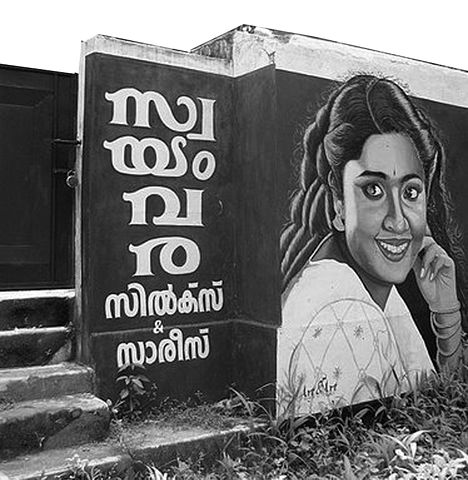
\includegraphics[width=\textwidth,height=8cm]{Kulasthree_Chapter_five_pic03.jpg}
\end{center}
%\caption*{പുലയർ - കെ പി പത്മനാഭ മേനോൻ - വാള്യം 3, (1929), 1984}
\end{figure}

\paragraph{}അതുപോലെ മരുമക്കത്തായക്കാരെല്ലാം നായന്മാരായിരുന്നില്ലെന്നും ഓർക്കണം. വടക്കേമലബാറിലെ തീയ്യർ, ഈഴവസമുദായത്തിലെ ചില വിഭാഗക്കാർ, മരുമക്കത്തായരീതി പിൻതുടർന്ന മാപ്പിളവിഭാഗക്കാർ, പുലയർ, മറ്റു കീഴാളജാതിക്കാർ, ഇവരെക്കൂടി എണ്ണിയിട്ടുവേണം മരുമക്കത്തായത്തെക്കുറിച്ചു പറയാൻ. ഇവരിൽ ആർക്കും നമ്പൂതിരിസംബന്ധം ഇല്ലായിരുന്നു; മേൽപ്പറഞ്ഞ പലവിധത്തിലുള്ള വിവാഹരീതികൾ ഇക്കൂട്ടരുടെയിടയിലും ഏകദേശം 20-ാം നൂറ്റാണ്ടിന്റെ പകുതിയോളവും ചിലയിടങ്ങളിൽ അതിനുശേഷവും നിലവിലുണ്ടായിരുന്നു.

\paragraph{}19-ാം നൂറ്റാണ്ടിന്റെ അവസാനഘട്ടത്തിൽ ഇംഗ്ലീഷ് വിദ്യാഭ്യാസം നേടിയ മരുമക്കത്തായികളിൽ പലർക്കും - ഇവർ അധികവും പുരുഷന്മാരായിരുന്നു - ഇത്തരം നടപ്പുരീതികളെക്കുറിച്ച് നാണക്കേടും അതൃപ്തിയും തോന്നിത്തുടങ്ങിയിരുന്നു. രണ്ടുതരം സ്വാധീനങ്ങളായിരുന്നു ഈ അഭിപ്രായത്തിനുപിന്നിൽ. ഒന്ന്, ആധുനികവിദ്യാഭ്യാസത്തിലൂടെ ഇന്ത്യയിലാകെ രൂപപ്പെട്ടുതുടങ്ങിയിരുന്ന പുതിയ മേൽജാതിസംസ്കാരത്തിന്റെ സ്വാധീനം. ബ്രാഹ്മണമൂല്യങ്ങൾക്ക് കണക്കിലധികം വില കല്പിക്കുകയും 'ഇന്ത്യൻസംസ്കൃതി'യുടെ അന്തഃസത്ത ബ്രാഹ്മണമൂല്യങ്ങളാണെന്ന് പ്രഖ്യാപിക്കുകയും ചെയ്ത ഈ പുതിയ പ്രവണത, മുൻ അദ്ധ്യായത്തിൽ സൂചിപ്പിച്ച 'പൗരസ്ത്യവാദി'കളിൽ > കാണുക പുറം 58 < ആരംഭിച്ച് പുതുവിദ്യാഭ്യാസം നേടിയ പുതിയ ഇന്ത്യൻ അധികാരിവർഗ്ഗത്തിലൂടെ വളർന്നു പന്തലിച്ചു. സ്ത്രീകളെ പൂർണ്ണമായും ഭർതൃകുടുംബത്തിന്റെ കീഴിലാക്കുന്ന, സ്ത്രീകൾക്ക് അവകാശങ്ങൾ അധികവും നിഷേധിക്കുന്ന, സ്വന്തം കുടുംബവുമായുള്ള അവരുടെ ബന്ധത്തെ അറുത്തുകളയുന്ന, വിവാഹംചെയ്യാത്ത സ്ത്രീക്ക് സമൂഹത്തിൽ അംഗത്വമില്ലെന്നുപോലും കരുതുന്ന ബ്രാഹ്മണ വിവാഹാദർശമാണ് 'ഇന്ത്യൻ വൈവാഹികസദാചാര'മെന്ന് ഈ പുതിയ ആശയവ്യവസ്ഥ സ്ഥാപിച്ചു. മദ്രാസിലും (ചെന്നൈ) മറ്റും ഉന്നതവിദ്യാഭ്യാസത്തിനായി എത്തിയ നായർയുവാക്കളിൽ പലരും ഇതിന്റെ സ്വാധീനത്തിലായി. മലബാറിൽ നിലവിലുള്ള വിവാഹം വെറും 'വെപ്പാട്ടിവ്യവസ്ഥ'യാണെന്ന് അവർ വാദിച്ചുതുടങ്ങി.




